Una búsqueda en profundidad (en inglés DFS o {\em Depth First Search}) es un algoritmo que permite recorrer todos los nodos de un grafo o árbol (teoría de grafos) de manera ordenada, pero no uniforme. Su funcionamiento consiste en ir expandiendo todos y cada uno de los nodos que va localizando, de forma recurrente, en un camino concreto. Cuando ya no quedan más nodos que visitar en dicho camino, regresa ({\em Backtracking}), de modo que repite el mismo proceso con cada uno de los hermanos del nodo ya procesado. 

El siguiente ejemplo ilustra el funcionamiento del algoritmo DFS sobre un grafo de ejemplo. El algoritmo comienza por el nodo 0.

\begin{figure}[h]
	\centering 
	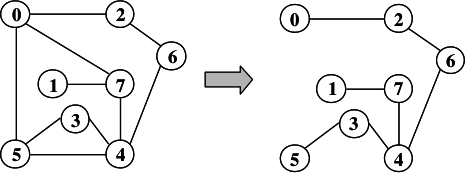
\includegraphics[scale=0.8]{img/dfs}
	\caption{Salida del DFS sobre el grafo.}
	\label{contexto:figura5}
\end{figure}

El pseudocódigo seria el siguiente:
\begin{lstlisting}[language=C++]
DFS(grafo G)     
  PARA CADA vertice u que pertenece V[G] HACER             
     estado[u] = NO_VISITADO             
     padre[u] = NULO     
     tiempo = 0     
     PARA CADA vertice u que pertenece V[G] HACER             
        SI estado[u] = NO_VISITADO ENTONCES                     
           DFS_Visitar(u,tiempo)
	
DFS_Visitar(nodo u, int tiempo)     
   estado[u] = VISITADO     
   tiempo = tiempo + 1     
   d[u] = tiempo     
   PARA CADA v que pertenece Vecinos[u] HACER             
      SI estado[v] = NO_VISITADO ENTONCES                     
         padre[v] = u                     
	     DFS_Visitar(v,tiempo)     
   estado[u] = TERMINADO     
   tiempo = tiempo + 1     
   f[u] = tiempo
\end{lstlisting} 

Como se puede observar esta variante es recursiva y es un ejemplo clásico de un {\em Backtracking} lo cual no es muy recomendable usar para grafos con una cantidad de nodos mayor de 9 nodos por la cantidad de operaciones que representa (9!), es por eso que se decide sustituir el elemento recursivo por una estructura de datos que puede simular la “recursividad” inicial del algoritmo y disminuye la complejidad del algoritmo. Dicha estructura es una pila

La idea detrás de DFS es profundizar lo más posible en el grafo y retroceder una vez que esté en un vértice sin vértices adyacentes no visitados.

Es muy fácil describir/implementar el algoritmo recursivamente: comenzamos la búsqueda en un vértice. Después de visitar un vértice, realizamos un DFS para cada vértice adyacente que no hayamos visitado antes. De esta manera visitamos todos los vértices que son alcanzables desde el vértice inicial.

Podemos clasificar las aristas usando el tiempo de entrada y salida de los nodos finales u y v de las aristas (u,v). Estas clasificaciones se usan a menudo para problemas como encontrar puentes y encontrar puntos de articulación.

Realizamos un DFS y clasificamos las aristas encontradas usando las siguientes reglas:

\begin{itemize}
	\item Si no se visita $v$: 
	\begin{itemize}
		\item Arista del árbol: si se visita $v$ después de $u$, entonces el borde $(u, v)$ se denomina arista del árbol. En otras palabras, si se visita $v$ por primera vez y se está visitando $u$ actualmente, entonces (u,v) se denomina arista del árbol. Estas aristas forman un árbol DFS y, por lo tanto, el nombre de arista del árbol.
		
	\end{itemize}
	\item Si se visita $v$ antes que $u$:
	\begin{itemize}
		\item Aristas posteriores: si $v$ es un antepasado de $u$, entonces el borde $(u, v)$ es una arista posterior. $v$ es un ancestro exactamente si ya ingresamos a $v$, pero aún no salimos de él. Las aristas posteriores completan un ciclo, ya que hay un camino desde el antepasado $v$ hasta el descendiente $u$ (en la recurrencia de DFS) y una arista desde el descendiente $u$ hasta el antepasado $v$ (arista posterior), por lo que se forma un ciclo. Los ciclos se pueden detectar usando aristas posteriores.
		
		\item Aristas delanteros: si $v$ es un descendiente de $u$, entonces el borde $(u,v)$ es una arista delantera. En otras palabras, si ya visitamos y salimos de $v$ y entrada[u]<entrada[v] entonces la arista (u,v) forma una arista delantero.
		
		\item Aristas cruzadas: si $v$ no es ni un ancestro ni un descendiente de $u$, entonces el borde (u,v) es uan arista cruzada. En otras palabras, si ya visitamos y salimos de $v$ y entrada[u]>entrada[v] entonces (u,v) es una arista cruzada.
	\end{itemize}
\end{itemize}

Nota: Las aristas delanteras y las aristas cruzadas solo existen en grafos dirigidos.